%% This is an example first chapter.  You should put chapter/appendix that you
%% write into a separate file, and add a line \include{yourfilename} to
%% main.tex, where `yourfilename.tex' is the name of the chapter/appendix file.
%% You can process specific files by typing their names in at the 
%% \files=
%% prompt when you run the file main.tex through LaTeX.
\chapter*{Introduction}
\addcontentsline{toc}{chapter}{Introduction}
The transition to sustainable energy, established on renewables and electric transport, critically depends on the development of efficient and affordable energy storage devices - rechargeable batteries. Among existing battery technologies Li-ion possesses many advantages in terms of specific energy, longevity, and power rate, explaining its fast penetration into portable electronics, electric cars, and even grid storage. 
One of the most prospective Li-ion technology is based on LiFePO$_4$ cathode material,  which combines high stability, safety, and affordability. However, the further improvement of this material, including full or partial replacement of Fe by Mn for an increase of voltage, requires better understanding and control of residual point defects left after synthesis.
Recently, it is shown with powder X-ray (PXRD) and neutron diffraction analysis, that hydrothermally synthesized LiFePO$_4$ (LFP) cathode material can have a deficiency in phosphorus, which should be highly unfavorable from the thermodynamic point of view~\cite{sumanov2019hydrotriphylites}. By careful analysis of iron oxidation states, Sumanov et al. suggested that some compensation mechanism should exist in P deficient LFP material. The infrared spectroscopy showed peaks from structural OH bonds, while thermogravimetric/mass-spectrometry analysis revealed the water loss by LFP sample in two stages with onsets at 350 and 450 $^\circ$C. Based on these results it was concluded that the compensation mechanism is related to the formation of structural OH defects, which can stabilize P vacancies. It was confirmed that the structural OH defects are not completely eliminated even up to 650 $^\circ$C. Sumanov et al. provided density functional calculations for PO$_4$/(OH)$_4$ substitutional defect, however they did not consider other possibilities for hydrogen insertions and substitutions. Therefore, the structure and energetics of OH-defects in LiFePO$_4$ material remain unclear. The complexity of the task is related to several degrees of freedom in PO$_4$/(OH)$_3$ and PO$_4$/(OH)$_4$ defects, which can result in numerous metastable configurations. Hence, the computational study of these defects should include global minima search approaches such as potential energy surface scan, while the defect stability should be studied with molecular dynamics at elevated temperatures.

The main aim of the current work is to determine the structure and energetics of OH defects in Li(Fe,Mn)PO$_4$ compounds using computational tools based on density functional theory.

To achieve the aim we set the following tasks:
\begin{enumerate} 
\item Calculate the energy and structure of OH defects in tetrahedral and octahedral voids of LiFePO$_4$;
\item Calculate the energy and structure of Li/H and Fe/2H substitution defects in LiFePO$_4$;
\item Construct full potential energy surface for PO$_4$/(OH)$_4$ substitution defect and calculate its formation energy and structure in Li(Fe,Mn)PO$_4$;
\item Study the dynamics and stability of PO$_4$/(OH)$_4$ defects in LiFePO$_4$ at elevated temperatures with ab initio molecular dynamics.
\end{enumerate}


% previously unknown OH-type defects, which have a detrimental effect on electrochemical properties~\cite{sumanov2019hydrotriphylites} . However, the direct observation of OH defect atomic structure was proved to be highly challenging with experimental techniques. 
% Most modern Li-ion batteries use LiFePO$_4$ material as a cathode in their construction. All physical properties of LiFePO$_4$ are widely investigated and known. The existing disadvantages are corrected with special synthesis conditions or coating, which makes a good operation features of LiFePO$_4$. Despite that, possible defects are still not well studied and their influence on the electrochemical characteristics is unknown. 
% According to previous investigation~\cite{sumanov2019hydrotriphylites} of a hydrothermally synthesized LiFePO$_4$ and its Powder X-ray (PXRD) and Neutron Diffraction analysis the phosphorus deficiency were obtained. At the same time the infrared spectroscopy shows the weak peak of hydrogen bond within the material, which is unusual for this structure. According to the study of the valence state of each atom in the structure, the substitution of phosphorus by hydrogen atoms is more plausible. But the structure and formation mechanism of this defect a quite difficult to study in experimental conditions. Density Functional Theory (DFT) and computational \textit{ab initio} tools are used in this application.

% Thus, the search for appropriate substitution positions of a hydrogen atom with relative energy was provided as a first step of research. As a next stage, the structure of hydrogen defect within an appropriate vacancy was found from the potential energy surface search. This result was additionally checked in molecular dynamics simulation. 
% Additionally, the influence of hydrogen defect to the electronic properties of structure was established. Finally, the influence of hydrogen substitution defect to lithium (de)intercalation process was studied.



% \newpage
\chapter{Review of Literature}
\section{Comparison of different battery systems and cathode materials}

An electric battery is one of the most important parts of modern electronic devices for everyday use.  There are two types of batteries: primary and secondary batteries. The first one is non- rechargeable and is discarded after single-use. In some cases such batteries are appropriate, for example in low-consuming electronics such as arm watches, where one battery can work for several years. However, in many cases primary batteries are still used in relatively high-power applications. The well-known example of high-load primary battery is an alkaline AA cell. It has a relatively small capacity of 700~mAh, and a low voltage of 1.5~V~\cite{david2001handbook}. The energy required to produce the battery is about 50 times greater than the battery stores itself. Moreover, such batteries are environmentally unfriendly. Therefore, whenever possible the primary batteries should be replaced with rechargeable analogs. 

There are several types of secondary batteries, like lead-acid, nickel-cadmium (Ni-Cd), nickel-metal hydride (Ni-MH), nickel-iron (Ni-Fe) and lithium-ion (Li-ion) battery. While every technology has its unique niche applications, the Li-ion has the highest energy density and the best longevity among them. As a result of that, several years ago Li-ion has become the only choice for smartphones and laptops, while becoming now to be the most popular energy storage technology in electric cars and even smart grids.  

The main components of a Li-ion battery are anode (a negative electrode with oxidation reaction), a cathode (a positive electrode with reduction reaction) and electronically non-conductive electrolyte. There is a lot of research related to the development of these components~\cite{wang2002investigation, ruess2017dye}. Below we focus on materials used for Li-ion cathode production. 

Several different materials are used as cathodes in Li-ion batteries. One of the most successful commercial cathode material is LiCoO$_2$ and was introduced in 1990. This material has  high voltage and high theoretical capacity  of 274 mAhg$^{-1}$; however the latter is reduced to the practical values of 140-160 mAhg$^{-1}$~\cite{luo2012binder}. To achieve higher capacities,  charging above 4.2V is required, which results in phase transformations from the hexagonal (R$\bar3$m) to the monoclinic structure, oxygen release and corresponding fast degradation~\cite{choi2002factors}. Overall, stability of the material is poor and thermal runaway is possible. Additionally, cobalt is quite expensive and its manufacture and recycling is environmentally unfriendly.

To achieve better parameters, several materials were identified as prospective cathodes: LiNiO$_2$, LiMn$_2$O$_4$, LiV$_3$O$_8$, LiMPO$_4$ (M = Fe, Mn, Co) and solid solutions like LiNi$_x$Co$_y$Mn$_z$O$_2$. For example LiNiO$_2$ has hexagonal structure R$\bar3$m, it provides practical capacity up to 200 mAhg$^{-1}$ at working voltage more than 4.8 V vs. Li$^+$/Li~\cite{amine2000olivine}. Additionally, such a cathode is less toxic and has a lower price compared to LiCoO$_2$. However, LiNiO$_2$ has the problems related to synthesis, safety and irreversible phase transformation. 
Another possible material is high-rate LiMn$_2$O$_4$ with spinel structure, which is less toxic and more economically favorable in comparison with LiCoO$_2$~\cite{yan1999microwave}. But due to its lower capacity (120 mAhg$^{-1}$) and limited life circle it does not correspond to modern requirements as well. 

The solid solutions  such as LiNi$_x$Co$_y$Mn$_z$O$_2$ can combine the advantages of single transition metal oxides described above. Such materials demonstrate practical capacities up to 220 mAhg$^{-1}$ and very good capacity retention up to 5000 cycles~\cite{salehen2017evaluation}. However, such materials still have relatively high prices and reduced thermal stability~\cite{elong2013solid}. 

Alternative oxide cathode materials are lithium trivanadate LiV$_3$O$_8$ (and other vanadium oxides), which has a high theoretical capacity (approximately 226 mAhg$^{-1}$~\cite{sun2010electrochemical}), relativity low cost and long life cycle. However low voltage of vanadium oxides prohibited their commercialization~\cite{liu2009effects}. 

One of the most economically viable material is LiFePO$_4$, which is based on the most abundant and cheap transition metal. This material was discovered in 1997 by Padhi et al.~\cite{padhi1997effect}. According to Padhi et al. and numerous following researches LiFePO$_4$ shows several advantages in comparison with oxide cathode materials. Firstly, LiFePO$_4$ has low toxicity and cheap due to the abundance of iron. Secondly, LiFePO$_4$ has higher thermal stability in a charged state with respect to phase transformations and oxygen evolution. Thirdly, it shows excellent cycling stability. 
The main disadvantage of LiFePO$_4$ is poor electronic conductivity, which is, however, solved by mixing with conductive carbon additive.
Despite lower working voltage and capacity
of LiFePO$_4$ compare to oxides, it has been commercialized and found application in electric buses and energy storage systems. 
The practical specific capacity, which is close to theoretical (till 170 mAhg$^{-1}$), combined with operating voltage of 3.5V gives practical
specific energies up to 580~Whkg$^{-1}$~\cite{franger2003comparison}. 

LiMnPO$_4$  has the same crystal structure and specific capacity as LiFePO$_4$, but posses a higher voltage of 4.1 eV vs. Li$^+$/Li, which gives a higher specific energy of 701 Whkg$^{-1}$~\cite{aravindan2013limnpo}. 
However, LiMnPO$_4$ is less stable then LiFePO$_4$ and suffers from structure disordering during cycling due to the Jahn-Teller effect. Also, LiMnPO$_4$ has slower ionic kinetics than LiFePO$_4$~\cite{yamada2006electrochemical}.
Besides that, there are numerous efforts~\cite{arvcon2004comparative,xu2017improvement} to overcome these limitations and create a new generation of cathodes based on LiMnPO$_4$ material.

\section{Crystal structure of LiFePO$_4$ and LiMnPO$_4$ material}

LiFePO$_4$, found in nature as triphylite mineral, has a crystal structure with $Pnma$ space group. This crystal structure is well known from studies on olivine minerals (Mg$_2$SiO$_4$) - widely present in Earth's mantle. Its framework consists of a slightly distorted hexagonal close-packed anion lattice with half of the octahedral sites occupied with Li and Fe and one-eighth of tetrahedral sites occupied by P. The lithium ions occupy the octahedral sites M$_1$ forming the edge-shared chains along the c-axes(Figure~\ref{ris:str} a)). The PO$_4$ tetrahedron makes the whole framework rigid  allowing Li deintercalation. The iron (or magnesium) atoms localize in zigzag chains of corner-shared octahedral sites M$_2$ parallel to the c-axes (Figure~\ref{ris:str} a)). The unit cell of LiFePO$_4$ and LiMnPO$_4$ is presented in Figure~\ref{ris:str} b). The experimental lattice constants for LiFePO$_4$ measured at 293K temperature  have the following values: a = 10.32 Å, b = 6.01 Å, and c = 4.69 Å \cite{urusova2017magnetic}. The lattice constants of LiMnPO$_4$ are: a = 10.445 Å, b = 6.10 Å, and c = 4.74 Å \cite{urusova2017magnetic}.

According to DFT calculations the barrier for Li vacancy migration along [010] direction is 0.3~eV~\cite{aksyonov2018understanding}. The migration pathway between adjacent lithium sites has a nonlinear curved shape. The same diffusion channels and pathway shape is observed for Li migration in LiMnPO$_4$, but the rate capability is lower due to higher Li vacancy - small polaron complexes formation energy and higher small polaron migration barriers~\cite{ong2011comparison}.

\begin{figure}[ht]
\begin{minipage}[h]{0.4\linewidth}
\center{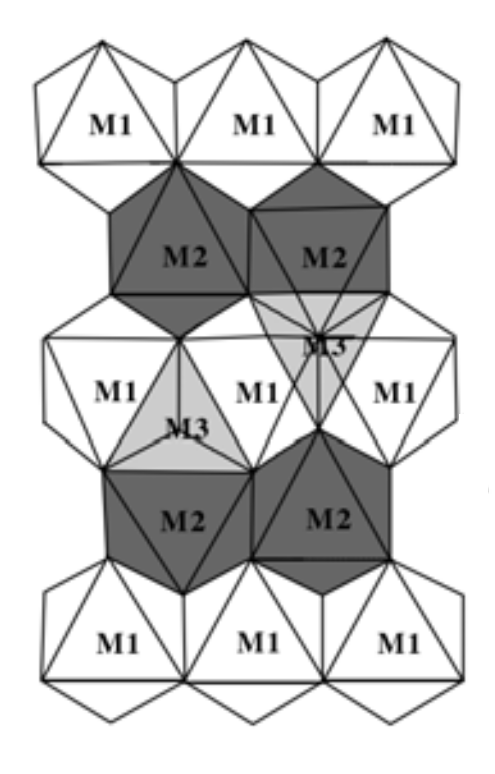
\includegraphics[width=0.8\linewidth]{pictures/LFP_schem_str.png}\\ a)}
\end{minipage}
\hfill
\begin{minipage}[h]{0.5\linewidth}
\center{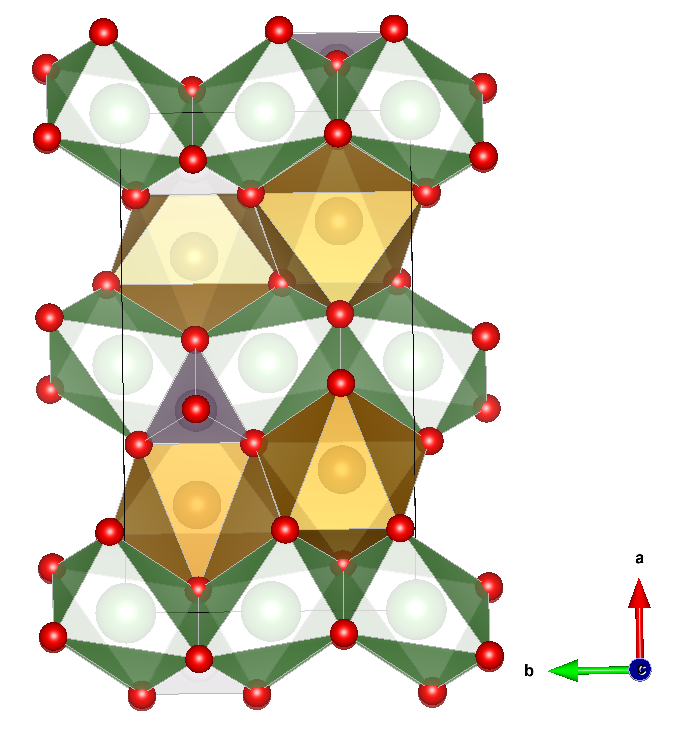
\includegraphics[width=0.9\linewidth]{pictures/LFP_xy.png}\\ b)}
\end{minipage}
\caption{Crystal structure of Li(Fe,Mn)PO$_4$ (a) ideal model; (b) schematic unit cell}
\label{ris:str}
\end{figure}

The main advantage of LiFe(Mn)PO$_4$ crystal structure is its thermodynamic and thermal stability even at temperatures above 200\textdegree C due to the strong P-O covalent bonds. The (PO$_4$)$^{3-}$ complexes are isolated from each other and touch the Fe octahedrons by sharing one of their edges. The deintercalation of Li$^+$ ions involves the change of iron oxidation states from Fe$^{2+}$ to Fe$^{3+}$ (or from Mn$^{2+}$ to Mn$^{3+}$ for LiMnPO$_4$) during the charge process without structural distortion. Since the energy level of Fe$^{2+}$/Fe$^{3+}$ redox couple lies lower by 3.5 eV with respect to the Fermi level of lithium (Figure~\ref{ris:3.5}), LiMnPO$_4$ based battery provides the operating voltage of 3.5~V versus Li/Li$^+$. In the case of LiMnPO$_4$ the working voltage is equal to 4.1 V \cite{zhou2017comparative}. 

\begin{figure}[ht]
\center{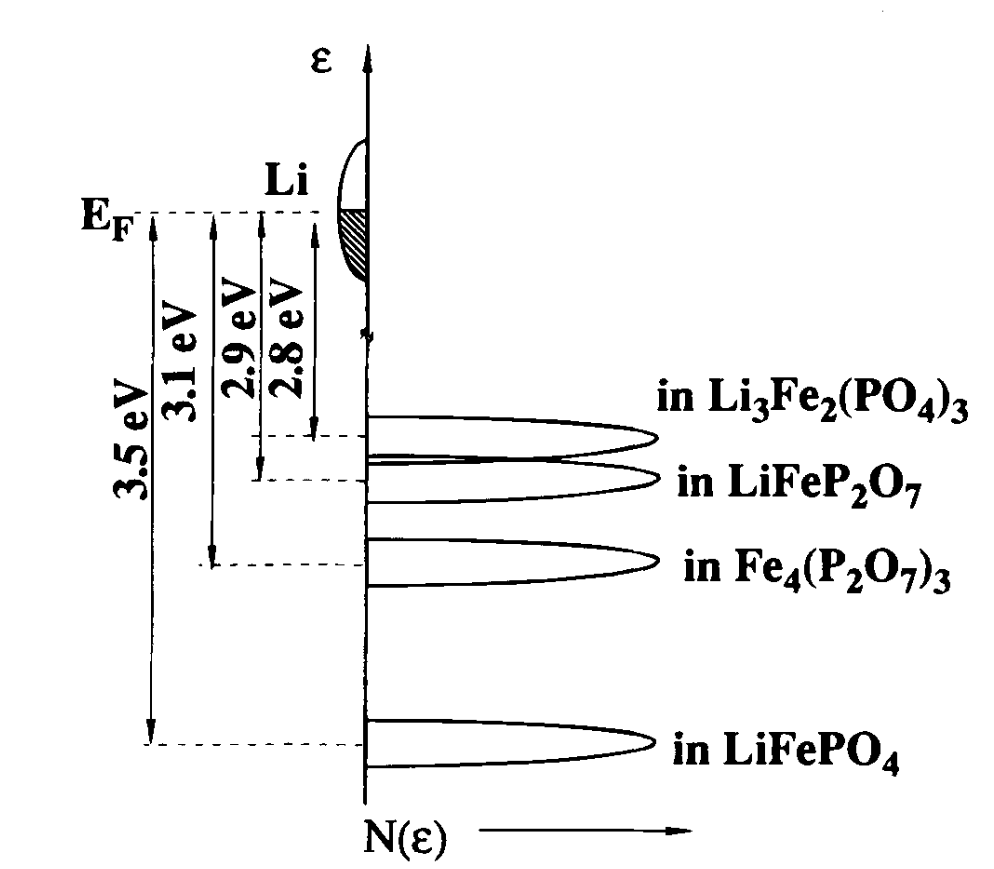
\includegraphics[width=0.7\linewidth]{pictures/LFP_3.5.png} a)}
\caption{Relative energy of Fe$^{2+}$/Fe$^{3+}$ redox couple in LiFePO$_4$ \cite{padhi1997effect}}
\label{ris:3.5}
\end{figure}

\section{Synthesis method for LiFePO$_4$ cathode material}

The material of Li(Fe,Mn)PO$_4$ can be produced using several synthesis methods \cite{wu2015lifepo4}. These include high-temperature solid-state method, sol-gel method, hydrothermal method and others. However, Li(Fe,Mn)PO$_4$ has low electric conductivity and relatively slow lithium-ion diffusion~\cite{padhi1997effect}, it is necessary to control the particle size during the synthesis process to shorten the [010] diffusion path for Li$^+$ ion and, thus, to improve the rate capability of Li(Fe,Mn)PO$_4$ \cite{huang2001approaching}. Additionally, highly dispersed carbonaceous materials can be added to Li(Fe,Mn)PO$_4$ in order to increase its electronic conductivity. The electrochemical activity of Li(Fe,Mn)PO$_4$ is strongly dependent on the preparation method. The hydrothermal method gives materials with high electrochemical properties, furthermore, it is simpler in use and energetically more efficient in comparison with alternative methods. Particles of LiFePO$_4$ are prepared by hydrothermal reaction from weak precursor solutions: LiOH, FeSO$_4$ and (NH$_4$)$_3$PO$_4$ in a molar ratio of 3:1:1. Precursors for LiMnPO$_4$ material synthesis are: Li$_2$SO$_4$, MnSO$_4$ and NH$_4$H$_2$PO$_4$, with a molar ratio of 3:1:1. After solutions mixing and heating in the Ar-atmosphere in autoclave at 230\textdegree C the resultant precipitation is collected and washed by water with ethanol and dried at 80\textdegree C in vacuum. The post-annealing process is necessary to perform at a high temperature above 500\textdegree C for 1 hour in order to achieve the crystallinity and enhance the electrochemical reactivity \cite{shiraishi2005formation}. 

\section{Electronic structure of LiFePO$_4$ and LiMnPO$_4$}

Due to low electric conductivity of LiFePO$_4$ it took more than 10 years to switch from research to the commercial production of cathodes. According to DFT calculations \cite{zaghib2007electronic}, the energy gaps for LiFePO$_4$ and FePO$_4$ are 3.7 eV and 1.9 eV, respectively, Figure~\ref{ris:LFPel}. The total density of states provided in this figure shows that the top of the valence band and bottom of the conduction band are occupied by electrons with the minority and majority spin channels, respectively.

% The Fe$^{2+}$ in LiFePO$_4$ is in the high spin S=2. Tts electronic configuration is t$_{2g}^4$e$_g^2$ with five electrons in spin up ($\uparrow$) and one electron in spin down ($\downarrow$) states (Fig.\ref{ris:LFPel}). 
\begin{figure}[ht]
\center{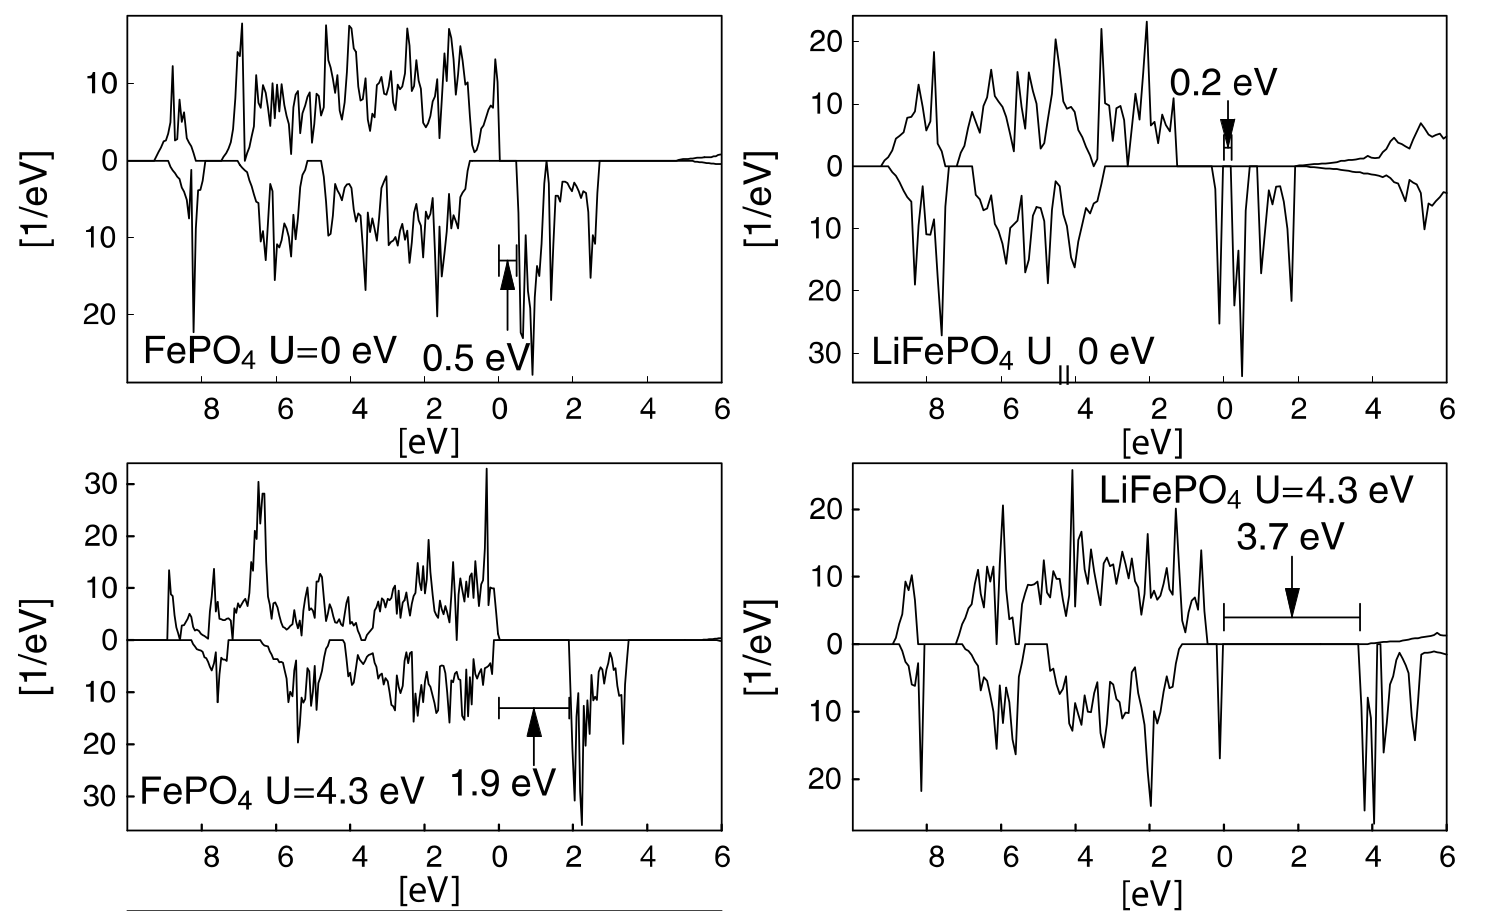
\includegraphics[width=0.9\linewidth]{pictures/LFP_el.png}}
\caption{Density of states of LiFePO$_4$ and FePO$_4$ in GGA and GGA+U methods}
\label{ris:LFPel}
\end{figure}

The Hubbard correction increases band gap of LiFePO$_4$ up to 3.7~eV, which is in  good alignment with experimental results~\cite{zaghib2007electronic}. The band gap for LiMnPO$_4$ is 3.8~eV (Figure~\ref{ris:LMPel}), which is also in good agreement with the experiment~\cite{zhang2019selecting}. Therefore, the correct description of electronic structure requires to use DFT+U method.

\begin{figure}[ht]
\center{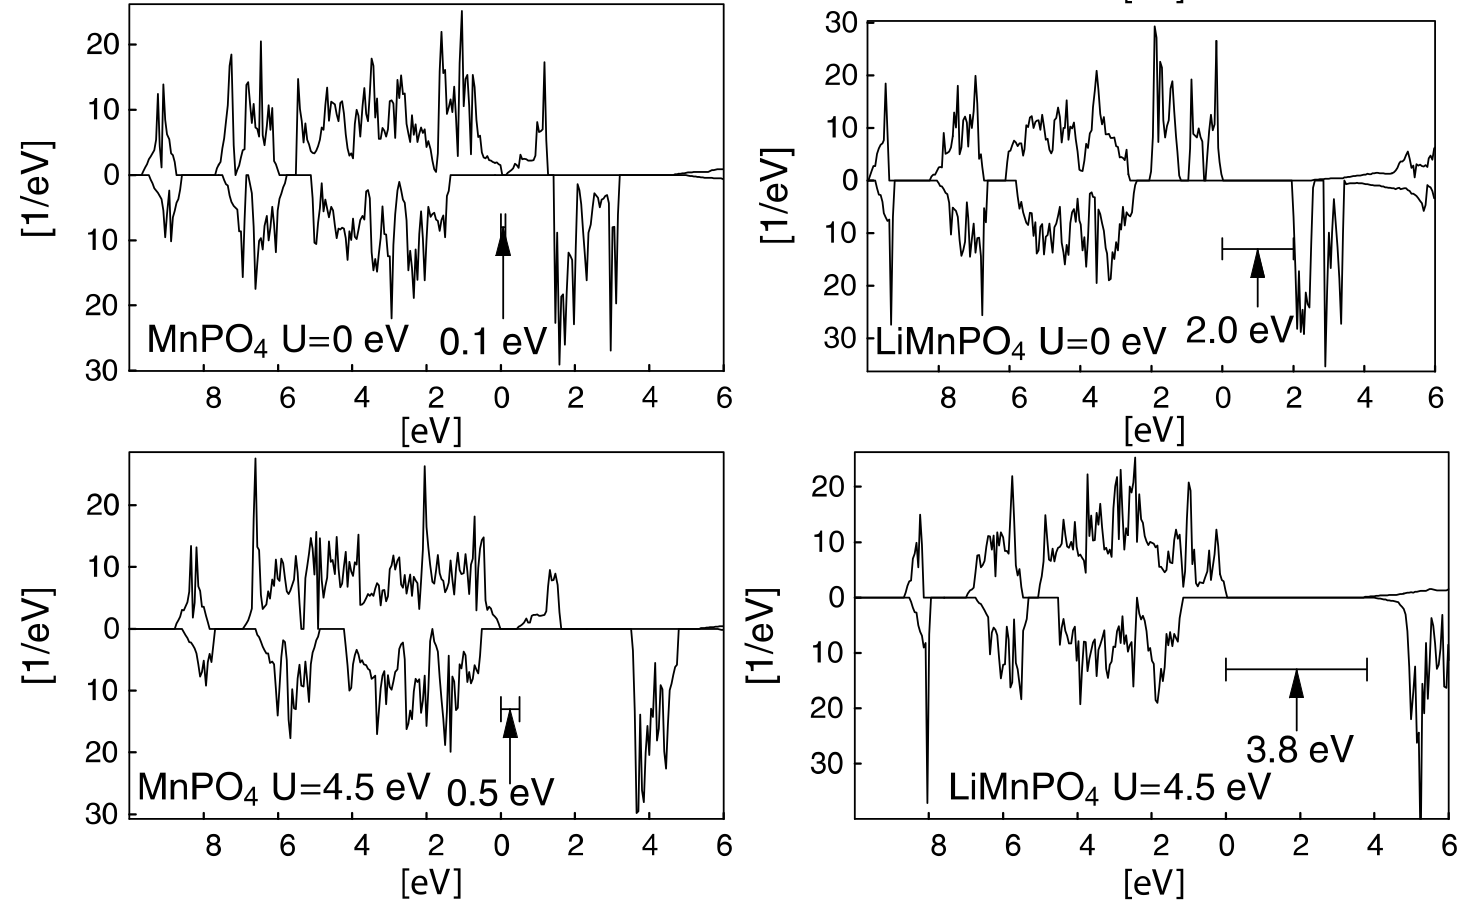
\includegraphics[width=0.9\linewidth]{pictures/LMP_el.png}}
\caption{Density of states of LiMnPO$_4$ and MnPO$_4$ in GGA and GGA+U methods}
\label{ris:LMPel}
\end{figure}

\section{Defects in LiFePO$_4$ and LiMnPO$_4$ cathode materials}

Though LiFePO$_4$ and LiMnPO$_4$ materials have a fairly simple crystal structure compared to other polyanionic compounds, investigation of defects in it is still a very important and active topic. The defects can have a huge influence on the electrochemical performance of the battery as a whole, and their study is critical for further material improvement. In literature, the majority of defect studies were conducted for LiFePO$_4$ rather than for LiMnPO$_4$. Below we provide a short review of the obtained results.

The antisite Li-Fe pair is an ‘intersite exchange’ point defect,  which is the most abundant point defect in LiFePO$_4$ material~\cite{islam2005atomic}. Islam et al. studied such antisite defects  using classical potentials and confirmed that among possible point defects it has the lowest formation energy~\cite{islam2005atomic}.
% The lithium and iron atoms are localized in M1 and M2 sites, respectively, (Fig.\ref{ris:str}).
The reason for low formation energy of antisite is related to close ionic radii of cations (0.76~\AA for Li$^+$ and 0.78~\AA for Fe$^{2+}$) and corresponding M-O distances. Indeed, the Fe-O and Li-O distances in LiFePO$_4$ are 2.150 \AA and 2.156~\AA, respectively. The antisite defect pairs Fe$^{\bullet}_{Li}$ - Li$^{\mapstochar}_{Fe}$ were directly observed in the experimental study with transmission electron microscopy \DA{check} \cite{paolella2015cation, chung2008atomic} and was identified in diffraction studies~\cite{chen2011situ}. Using DFT calculations the aggregation of Li-Fe antisite pairs was established for LiFePO$_4$, while no agregation was found in LiMnPO$_4$~\cite{chung2012distinct}. 

It is considered that antisite defects reduce ionic conductivity of Li(Fe,Mn)PO$_4$ by blocking Li$^+$ [010] diffusion channels by Fe$^{2+}$ or Mn$^{2+}$) cations. Also, part of Li$^+$ is becoming  electrochemically inactive, which reduces specific capacity of material. To reduce the amount of Li-Fe antisite defects the special measures are undertaken during the synthesis. In particular, a post-heat treatment at 500\textdegree C~\cite{chen2011study} results in defects recombination. Also, it is shown that nanosized powder of LFP contains less amount of antisite defects~\cite{jensen2013defects}.

% The second possibility of observing an iron atom in M1 place is the doping of material with iron atoms in lithium vacancy sites Fe$^{\bullet}_{Li}$ - V$^{\mapstochar}_{Li}$. There is a relatively low formation energy of Frenkel lithium defect \cite{islam2005atomic}. 

The removal of one Li results in a negatively charged V$^{\mapstochar}_{Li}$, which is compensated by the change of the Fe oxidation state from +2 to +3 with the formation of small polaron~\cite{axmann2009nonstoichiometric}. 
% Additionally, this type of defect also contributes to the blocking of Li-transport through the material, which has a negative effect on the electrochemical properties of the cathode. 
% Overall, there are significant efforts to control the defect composition in LiFePO$_4$ by modifying the synthesis and processing conditions~\cite{halankar2018optimization}.

The last possible defect we like to cover is the phosphorus vacancy, which should have relatively high energy of formation and very small concentrations. However, non-negligible deficiency of P  was observed in LiFePO$_4$ experimentally~\cite{amisse2015singular}. Sumanov et al. suggested that the P deficiency in hydrothermally synthesized LiFePO$_4$ can be explained by partial replacement of PO$^4_{3-}$ polyanion by four hydroxyl groups~\cite{sumanov2019hydrotriphylites}. In their work, the LiFePO$_4$ samples were prepared from the aqueous solutions with a low concentration of initial reagents: H$_3$PO$_4$, LiOH·H$_2$O, FeSO$_4$·7H$_2$O, and ascorbic acid taken in the 1:3:1:1 molar ratio, in water (just to maximize the amount of the defects). Using the Powder X-ray (PXRD) and Neutron Diffraction analysis the presence of the antisite Li-Fe defects and phosphorus deficiency were determined. Additionally, the change of iron oxidation state from Fe$^{2+}$ to Fe$^{3+}$ was identified. Among a series of samples, for example, in the case of Li$_{0.93}$Fe$_{1.07}$P$_{0.84}$O$_4$, the PXRD determined composition implies that 68$\%$ of Fe should be in Fe$^{3+}$ state for charge balance. However the M{\"o}ssbauer spectroscopy shows the only 4$\%$ of Fe is in Fe$^{3+}$ state. Such behavior indicates that some charge compensation mechanism should exists. The infrared (IR)-spectroscopy showed the presence of OH-bonds within the crystal, which allowed to assume that P deficiency is caused by OH defects. The structure of OH-defects in LiFePO$_4$ cannot be determined from the experiment, therefore their computational study is required. Accurate knowledge of hydrogen positions within the phosphorus vacancy as well as their formation energies can be obtained with density functional theory (DFT) computations. 



\section{OH defects in olivine (Mg, Fe)SiO$_4$ minerals}
LiFePO$_4$ share the same crystal structure with olivine mineral with typical formula (Mg, Fe)SiO$_4$. This mineral is abundant in Earth mantle and was extensively studied previously. In particular, it is well established that olivine minerals contains significant amount of structural water \DA{add refs}. 
% Each of material under investigation LiFePO$_4$ and LiMnPO$_4$ has a triphylite unit cell type with general formula Li$M$PO$_4$ adopts the olivine structure M$_2$XO$_4$. It is well known that olivine material is strongly affected by the trace amounts of water. 
It is confirmed that hydrogen resides as a substitution defect in place of Fe or Si sites forming OH groups \DA{add refs}. 
% Such hydrogen defects influence the chemical and physical properties of the material, including electrical conductivity.
The best investigated material in terms of OH defects is Mg$_2$SiO$_4$, where Si or Mg atom is replaced with four or two hydrogen atoms \cite{wright1994computer}. 
% The study of structures with incorporation hydrogen atoms was done both experimentally and computationally. 
The presence of OH defects within the structure of Mg$_2$SiO$_4$ was confirmed by IR-spectroscopy studies \cite{rossman1996studies}. 
% And, in this application, the formation mechanism of OH bonds is under investigation. 
According to ab initio calculations \cite{brodholt2000ab}, the formation energy of Si vacancy is lower than that of Mg vacancy in Mg$_2$SiO$_4$. 
% But the diffusion path of silicon from its tetrahedral site is through interstitial mechanism with higher energy. In case of vacancy observation on magnesium site the diffusion path passes through the jumping between adjacent octahedral magnesium sites since they are connected either by faces or edges. Thus, the silicon-vacancy formation is a minor defect, but the presence of hydrogen atoms at the silicon-vacancy site can be described in terms of the exchange mechanism between silicon and hydrogen with a decrease of its formation energy. Finally, the mechanism of vacancy formation in dry olivine is quite different from aqueous mineral and the availability of hydrogen defect on the silicon site is energetically more favorable, which was approved at the experiment. These results are important in the framework of fundamental knowledge about the mechanism of hydrogen defect formation within the olivine materials.
However, it was not clear for a long time whether H substitute Mg or Si in Mg$_2$SiO$_4$. Only in the recent study it was established that both cases are possible depending on temperature and pressure~\cite{qin2018ab}

In the case of LiFePO$_4$ the situation is even more complicated, since hydrogen can replace three species: Li, Fe, or P. Moreover, LiFePO$_4$ lattice contains 5 tetrahedral and 2 octahedral non-equivalent voids per formula unit, each of them can be a suitable alternative for hydrogen position. 

